\documentclass[10pt,
               a4paper,
               journal,
               ]{IEEEtran}
\makeatletter

\def\markboth#1#2{\def\leftmark{\@IEEEcompsoconly{\sffamily}\MakeUppercase{\protect#1}}%
\def\rightmark{\@IEEEcompsoconly{\sffamily}\MakeUppercase{\protect#2}}}
\makeatother

\usepackage[utf8]{inputenc}
\usepackage[T1]{fontenc}
\usepackage{cite}
\usepackage{amsfonts}
\usepackage[pdftex]{graphicx}
\graphicspath{{../png/}}
\DeclareGraphicsExtensions{.png}
\usepackage[cmex10]{amsmath}
\interdisplaylinepenalty=2500
\usepackage{algorithmic}
\usepackage{array}
\usepackage{mdwmath}
\usepackage{mdwtab}
\usepackage{eqparbox}
\usepackage[caption=false,font=footnotesize]{subfig}
\usepackage{fixltx2e}
\usepackage{stfloats}
\usepackage{url}
\hyphenation{op-tical net-works semi-conduc-tor}
\usepackage{tikz}
\usepackage{listings}
\usepackage{color}

\definecolor{dkgreen}{rgb}{0,0.6,0}
\definecolor{gray}{rgb}{0.5,0.5,0.5}
\definecolor{mauve}{rgb}{0.58,0,0.82}

\lstset{frame=tb,
  language=C++,
  aboveskip=3mm,
  belowskip=3mm,
  showstringspaces=false,
  columns=flexible,
  basicstyle={\small\ttfamily},
  numbers=none,
  numberstyle=\tiny\color{gray},
  keywordstyle=\color{blue},
  commentstyle=\color{dkgreen},
  stringstyle=\color{mauve},
  breaklines=true,
  breakatwhitespace=true
  tabsize=3
}

\begin{document}
	\title{Constraint Programming - Inside Gecode}
	\author{Benedikt~Schmidt}
	\markboth{Advanced Seminar for Security in Information Technology, Summer Term 2014}%
	{Benedikt Schmidt: Constraint Programming - Inside Gecode}	
	\maketitle	
	
	\begin{abstract}	
		\textit{last thing to write}	
	\end{abstract}
	
	\section{Introduction}
	Constraint programming is a tool to solve mathematical problems through the formulation of constraints, which describe the desired solution. As typically a foraml and exact definition, like it can be found in \cite[p. 16]{handbookCP} for constraint propagation, is not as helpful as an example, I would like to give you a short overview on the topic through the well known problem \emph{SEND MORE MONEY}.
	
	Consider the problem
	\[SEND + MORE = MONEY\]
	where every character is a variable and the position in the word describes the weight.
	\begin{equation}
	\label{eq:linearConstraint}
	\begin{split}
		& S \cdot 10^3 + E \cdot 10^2 + N \cdot 10^1 + D \cdot 10^0 + \\ 
		& M \cdot 10^3 + O \cdot 10^2 + R \cdot 10^1 + E \cdot 10^0 = \\ 
		& M \cdot 10^4 + O \cdot 10^3 + N \cdot 10^2 + E \cdot 10^1 + Y \cdot 10^0
	\end{split}
	\end{equation}		
	
	To narrow the solution space a little bit down I state additional constraints:
	\begin{enumerate}
	\item All variables must have different values.
		\begin{equation}
		\begin{split}
			S \ne E \land S \ne N \land & S \ne D \land \dots \land \\
			E \ne N \land & E \ne D \land \dots \land \\
			& N \ne D \land \dots
		\end{split}
		\end{equation}	
	\item There must not be a trailing zero. Combined with the so-called all-different constraint \cite{allDifferent} from above this results in
		\begin{equation}
			S \ne 0 \land M \ne 0
		\end{equation}
	\end{enumerate}
	
	Now a solver for constraint programming like Gecode provides the necessary tools to define these constraints in their most natural form as equations and inequations and will find all possible solutions or just one of them, depending on the selected search algorithm. Actually this example contains only linear constraints and could therefore be solved through linear programming. As linear programming is only a subset of constraint programming the latter one is often the more useful one, because not every problem in the real world is linear or can be linearized in a useful way. Consequently constraint programming with its ability to consider constraints in there most general form can be used in various fields like scheduling of resources, computer-aided design and robotics \cite[p. 221]{trendsInCP}.
	
	In the following I will describe the necessary steps to solve a problem with constraint programming and as example of an implementation I will always refer to \emph{Gecode} \cite{gecode}.
	
	\section{State of the Art}
	\subsection{Variable Domains}
	In constraint programming to a variable a set of possible values is connected, the so called domain. This domain can be a finite or inifite set of integers, true or false and intervals. Depending on the domain a variable is called an integer, boolean or floating variable. Possible ranges for a variable $x$ of each domain are:
	\begin{itemize}
		\item Integer: $x \in \mathbb{N}$, $x \in \{-5, 4, 10\}$, \dots
		\item Bool: $x \in \{\text{true}, \text{false}\}$
		\item Float: $x \in [-4, 3]$, $x \in [-10, 8] \cup [10, 12]$, \dots
	\end{itemize}
	This distinction is important as especially for floating variables the classical approach to constraint programming, a backtrack search, can not be applied directly. For integer and boolean variables the domain for each variable is reduced step by step during a search, either by constraints which rule out certain values or by trial and error. As floating variables do not have discrete values for their domains the procedere in this case is to reduce or split intervals based on constraints or to apply trial and error through splitting the intervals \cite[p. 571]{handbookCP}. I will come back to this topic later during the discussion of the branch-and-bound search.
	
	\subsection{Constraint Types}
	As already mentioned before constraint programming is the generalization of linear programming, therefore it is at least possible do define linear constraints like [equation \ref{eq:linearConstraint}]. Which statements are possible to make varies than very much from the programming language in which the problem is implemented and the used toolset. Typical constraints would be
	\begin{itemize}
		\item Equalities: $x = y + 2$, $x^2 + y^2 = 1$, \dots
		\item Inequalities: $x \ne y$, \dots
		\item Relations: $x < 2 y$, $e^x < 4$, \dots
	\end{itemize}
	In Gecode for example it is very easy to create for example a nonlinear constraint based on the integer variables a, b, c and d \cite[p. 120]{programmingGecode}:
	\begin{lstlisting}
rel(home, a+b*(c+d) == 0);
	\end{lstlisting}
	This single statement in C++ implements the constraint
	\begin{equation}
		a + b \cdot (c + d) == 0
	\end{equation}
	what is a quite handy way to do it.
	
	\begin{figure}
	\center
	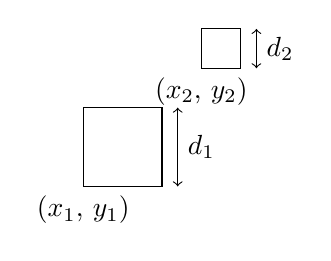
\begin{tikzpicture}
		\draw (0, 0) rectangle (1, 1);
		\node at (0, -0.3) {($x_1$, $y_1$)};
		\draw[arrows=<->] (1.2, 0) -- (1.2, 1);
		\node at (1.5, 0.5) {$d_1$};
		\draw (1.5, 1.5) rectangle(2, 2);
		\node at (1.5, 1.2) {($x_2$, $y_2$)};
		\draw[arrows=<->] (2.2, 1.5) -- (2.2, 2);
		\node at (2.5, 1.75) {$d_2$};
	\end{tikzpicture}
	\caption{two squares which should not overlap}
	\label{fig:squares}
	\end{figure}
	Hence there are boolean variables available it is also possible to use logical operators to combine other constraint types to logical expressions. To show the usage of this on an example I will give the implementation for the placement of two squares such that they do not overlap [figure \ref{fig:squares}]. This problem can be expressed mathematically by \cite[p. 101]{programmingGecode}
	\begin{equation}
	\begin{split}
		x_1 + d_1 \le x_2 & \lor x_2 + d_2 \le x_1 \lor \\
		y_1 + d_1 \le y_2 & \lor y_2 + d_2 \le y_1
	\end{split}
	\end{equation}
	and in Gecode by
	\begin{lstlisting}
rel(home,	(x1 + d1 <= x2) || 
		(x2 + d2 <= x1) || 
		(y1 + d1 <= y2) || 
		(y2 + d2 <= y1));
	\end{lstlisting}
	which is again quite obvious to a reader with some experience in a C-like programming language.	
	
	\subsection{Constraint Propagation}
	
	\subsection{Search Algorithms}
	
	\section{Conclusion}
	\textit{conclusion}
	
	\begin{thebibliography}{1}
		\bibitem{handbookCP}
		F.~Rossi, P.van~Beek and T.Walsh, \emph{Handbook of Constraint Programming}, Amsterdam, The Netherlands: Elsevier, 2006, ISBN: 978-0-444-52726-4
		\bibitem{allDifferent}
		W.~van~Hoeve, \emph{The Alldifferent Constraint: A Survey}, http://www.andrew.cmu.edu/user/vanhoeve/papers/alldiff.pdf
		\bibitem{trendsInCP}
		F.~Benhamou, N.~Jussien, B.A.O'Sullivan, \emph{Trends in Constraint Programming}, Wiley-ISTE, 2007, ISBN: 978-1-905209-97-2
		\bibitem{gecode}
		http://www.gecode.org/
		\bibitem{programmingGecode}
		C.~Schulte, G.~Tack and M.Z.Lagerkvist, \emph{Modeling and Programming with Gecode}, http://www.gecode.org/doc-latest/MPG.pdf
	\end{thebibliography}
\end{document}


